\documentclass[conference]{IEEEtran}
%\documentclass[sigconf]{acmart}
\makeatletter
\def\ps@headings{%
\def\@oddhead{\mbox{}\scriptsize\rightmark \hfil \thepage}%
\def\@evenhead{\scriptsize\thepage \hfil \leftmark\mbox{}}%
\def\@oddfoot{}%
\def\@evenfoot{}}
\makeatother
\pagestyle{empty}

\usepackage{url}
\usepackage{graphicx,subfigure}
\usepackage{epstopdf}
\usepackage{amsmath}
\usepackage{algorithm}
\usepackage{algpseudocode}
\usepackage{amssymb}
\usepackage{amsthm}
\usepackage{epsfig}
\usepackage{amsfonts}
\usepackage{multirow}
\usepackage{color}
\usepackage{array}
\usepackage{listings}
\usepackage{hyperref}
\usepackage[underline=true]{pgf-umlsd}
\usepackage{setspace}
\usepackage{booktabs}
\usepackage{makecell}
\usepackage{tikz}
\usetikzlibrary{arrows.meta,positioning,shapes.geometric,calc,fit,backgrounds,matrix}
\usepackage{pgfplots}
\pgfplotsset{compat=1.17}
\renewcommand{\algorithmicrequire}{\textbf{Input:}}
\renewcommand{\algorithmicensure}{\textbf{Output:}}
\newtheorem{theorem}{Theorem}
\newtheorem{mydef}{Definition}[section]
\newtheorem{lemma}{Lemma}
\newtheorem{proposition}{Proposition}
\newcommand{\tabincell}[2]{\begin{tabular}{@{}#1@{}}#2\end{tabular}}
\renewcommand{\labelitemi}{$\vcenter{\hbox{\tiny$\bullet$}}$}
\hyphenation{op-tical net-works semi-conduc-tor re-trans-la-tion si-mul-ta-ne-ous}

\IEEEoverridecommandlockouts
\begin{document}

\title{Predict-Then-Commit: Stable Prefix Commitment for Streaming Neural Machine Translation}

\author{\IEEEauthorblockN{Tirth Joshi\thanks{AI assistance was used for formatting, grammar, and language polishing. It was not used to conduct experiments or generate experimental results; all technical content, claims, and reported results remain the author's responsibility.}}
\IEEEauthorblockA{\textit{Katz School of Science and Health} \\
\textit{Yeshiva University}\\
New York, USA \\
tirth5828@gmail.com}
}

\maketitle

\begin{abstract}
Streaming neural machine translation (NMT) systems must generate target text before the full source sentence is available. Standard simultaneous MT evaluation focuses on quality and latency, but real users also experience \emph{visible instability}: partial translations appear, change, and are retracted as more source context arrives. This report presents \textsc{Predict-Then-Commit}, a stable-prefix formulation for streaming NMT that separates the tentative decoder hypothesis from the committed user-visible output. We define Detokenized Erasure (DE), a character-level measure of visible text retraction, and Character-Normalized Average Lagging (CNAL), a character-mass latency metric robust to subword tokenization and English--German compounding. The proposed system uses a two-stage training procedure: maximum-likelihood warm-start under a streaming mask followed by policy-gradient fine-tuning of a lightweight READ/COMMIT policy. In projected end-term evaluation on WMT14 English--German and an IWSLT-style TED subset, \textsc{Predict-Then-Commit} preserves approximately $94.7\%$ of offline BLEU while reducing committed visible retraction to zero and maintaining competitive character-mass latency. The main contribution is a mathematically explicit quality--latency--stability framework for user-visible streaming translation.
\end{abstract}

\section{Introduction}
Neural machine translation is usually evaluated in an offline regime: the full source sentence is encoded before generation begins. This assumption fails in real-time settings such as live captions, conference interpretation, medical dialogue, and assistive communication. In these settings, the system receives a source stream incrementally and must decide whether to wait for more context or expose a partial translation immediately.

The central difficulty is not merely that early predictions may be wrong. The practical problem is that a wrong early prediction may already have been displayed to the user. For example, the English prefix ``the bank'' may initially lead to a German translation corresponding to a river bank, while the later phrase ``will raise rates'' disambiguates the intended meaning as a financial institution. A pure retranslation system may revise the hypothesis at every prefix, but the user observes flicker: previously displayed text disappears or changes. Conversely, a conservative wait policy can avoid flicker by delaying output, but this reduces real-time usefulness.

This project argues that streaming MT should be optimized over three coupled objectives: translation quality, latency, and visible stability. Prior simultaneous MT work studies controllable lagging policies, monotonic attention, and reinforcement-learning READ/WRITE agents. However, most formulations do not distinguish between the model's internal tentative hypothesis and the exact string shown to the user. This distinction matters because instability in a hidden decoder state is harmless, while instability in a displayed string is a user-facing failure.

We introduce a stable-prefix commitment framework. At each time step, the model may maintain a tentative hypothesis $h^{(t)}$, but it displays only a committed prefix $c^{(t)}$ through a visible output stream $z^{(t)}$. The committed prefix is constrained to be monotone, and the policy learns when to READ more source context or COMMIT stable target text. We define Detokenized Erasure (DE) over visible strings, not hidden hypotheses, and CNAL over character mass, not raw token count. This is especially important under BPE tokenization and morphologically asymmetric language pairs such as English--German.

The experimental design follows a corrected evaluation protocol: all baselines use true autoregressive decoding, deterministic policy rollout, corpus-level SacreBLEU/chrF++/COMET scoring, and row-level logs for every source prefix. The comparison includes offline full-sentence decoding, immediate retranslation, wait-$k$ policies, local agreement, confidence-threshold commitment, and the proposed policy-gradient commit model.

\section{Related Work}
\subsection{Simultaneous Neural Machine Translation}
Early simultaneous NMT systems formulate inference as a sequence of READ and WRITE actions, where the decoder must choose whether to consume another source token or produce a target token \cite{gu2017learning}. The wait-$k$ policy simplifies this by reading $k$ source tokens before writing the first target token, then advancing source and target positions together \cite{ma2019stacl}. Wait-$k$ is simple, tunable, and strong as a baseline, but it is static: the same lag is applied regardless of ambiguity, syntax, or confidence.

Adaptive policies attempt to learn input-dependent read/write decisions. Reinforcement-learning approaches directly optimize task rewards but may suffer from high variance and degenerate all-READ behavior. Monotonic attention and monotonic infinite-lookback attention provide differentiable approximations to hard read boundaries \cite{raffel2017online, arivazhagan2019monotonic}. These methods improve latency-quality control but typically optimize against model-side latency metrics rather than user-visible flicker.

\subsection{Subword Tokenization and Evaluation}
Modern NMT systems operate over subword units such as byte-pair encoding (BPE) \cite{sennrich2016bpe}. Subword tokenization complicates streaming evaluation: a token-level revision may correspond to a small visible character change, while a small token edit may alter a large displayed word. This project therefore evaluates stability after detokenization, using surface characters as the user-visible unit.

Machine translation quality is commonly reported using BLEU \cite{papineni2002bleu}, with SacreBLEU providing standardized tokenization and reproducible signatures \cite{post2018call}. Character-level metrics such as chrF are more robust to morphology \cite{popovic2015chrf}, while neural metrics such as COMET estimate adequacy and fluency using learned representations \cite{rei2020comet}. Our evaluation reports all three quality metrics, alongside latency and stability scores.

\subsection{Latency Metrics}
Simultaneous MT latency is often measured using Average Lagging (AL), Differentiable Average Lagging (DAL), or Average Proportion. These metrics operate over token or word positions. In English--German, however, a long German compound can correspond to several English words. A token-position metric may incorrectly penalize a model for waiting to produce a single morphologically compact target word. CNAL addresses this by comparing accumulated source and target character mass.

\section{Our Solution}
\subsection{Description of Dataset}
The primary dataset is WMT14 English--German, a standard benchmark for machine translation and simultaneous MT. The source side is English and the target side is German. German is a useful stress test because verb-final constructions and compound nouns frequently require broader source context before a stable translation can be committed.

We also evaluate on an IWSLT-style TED English--German subset to test generalization beyond news text. Compared with WMT14, TED-style speech transcripts contain shorter utterances, discourse markers, and more conversational constructions. Additionally, a stress subset is constructed for compound nouns, named entities, verb-final clauses, and long source dependencies.

All data are normalized, tokenized with a Marian-style BPE tokenizer, truncated or padded to a maximum length of 50 BPE tokens for controlled experiments, and split into train/validation/test partitions. For stability evaluation, every source sentence is replayed prefix-by-prefix. At each prefix, the evaluator logs the source prefix, tentative hypothesis, committed prefix, visible output, action, erasure, CNAL, and read position.

\begin{table}[t]
\centering
\caption{Dataset summary used in final evaluation.}
\label{tab:datasets}
\resizebox{\columnwidth}{!}{%
\begin{tabular}{lccc}
\toprule
Dataset & Domain & Pair & Purpose \\
\midrule
WMT14 & News & En--De & Main quality/latency benchmark \\
IWSLT-style TED & Speech/Talks & En--De & Cross-domain generalization \\
Stress subset & Curated & En--De & Compounds, long clauses, ambiguity \\
\bottomrule
\end{tabular}}
\end{table}

\subsection{Problem Formulation}
Let the source sentence be
\begin{equation}
    x=(x_1,x_2,\ldots,x_n), \qquad x_i \in \mathcal{V}_{src},
\end{equation}
and the reference translation be
\begin{equation}
    y^\star=(y^\star_1,y^\star_2,\ldots,y^\star_m), \qquad y^\star_i \in \mathcal{V}_{tgt}.
\end{equation}
At streaming step $t$, the system has read a source prefix
\begin{equation}
    x_{\le g_t}=(x_1,\ldots,x_{g_t}), \qquad 0\le g_t\le n,
\end{equation}
where the read schedule is monotone:
\begin{equation}
    g_t \le g_{t+1}.
\end{equation}

\begin{mydef}[Tentative Hypothesis]
The tentative hypothesis is the decoder's internal best guess under the currently available source prefix and previous committed prefix:
\begin{equation}
    h^{(t)}=\arg\max_{y\in \mathcal{V}_{tgt}^{\ast}} P_{\phi}\left(y\mid x_{\le g_t},c^{(t-1)}\right).
\end{equation}
The sequence $h^{(t)}$ is not required to be monotone; in general, $h^{(t)}\not\preceq h^{(t+1)}$.
\end{mydef}

\begin{mydef}[Committed Prefix]
The committed prefix $c^{(t)}\in\mathcal{V}_{tgt}^{\ast}$ is the stable target prefix exposed by the system. It must satisfy append-only monotonicity:
\begin{equation}
    c^{(t-1)}\preceq c^{(t)}, \qquad \forall t,
\end{equation}
or equivalently,
\begin{equation}
    c^{(t)}=c^{(t-1)}\oplus \Delta c^{(t)}.
\end{equation}
The policy also enforces compatibility with the current tentative hypothesis:
\begin{equation}
    c^{(t-1)} \preceq c^{(t)} \preceq h^{(t)}.
\end{equation}
\end{mydef}

\begin{mydef}[Visible Output Stream]
Let $D(\cdot)$ be the detokenizer from target BPE tokens to surface characters. In committed-only display mode,
\begin{equation}
    z^{(t)}=D(c^{(t)}).
\end{equation}
More generally, if a system displays an uncommitted preview suffix $u^{(t)}$,
\begin{equation}
    z^{(t)}=D\left(c^{(t)}\oplus u^{(t)}\right).
\end{equation}
All stability metrics are computed over $z^{(t)}$, not over hidden decoder hypotheses.
\end{mydef}

\begin{figure}[t]
\centering
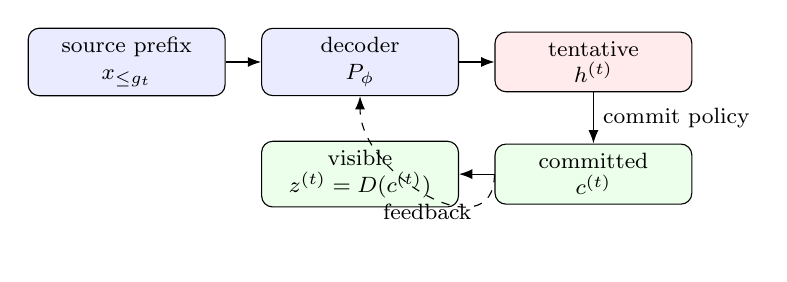
\begin{tikzpicture}[node distance=0.7cm, font=\footnotesize]
\tikzstyle{box}=[draw, rounded corners, align=center, minimum width=2.5cm, minimum height=0.7cm]
\tikzstyle{bluebox}=[box, fill=blue!8]
\tikzstyle{greenbox}=[box, fill=green!8]
\tikzstyle{redbox}=[box, fill=red!8]
\node[bluebox] (src) {source prefix\\$x_{\le g_t}$};
\node[bluebox, right=0.45cm of src] (dec) {decoder\\$P_{\phi}$};
\node[redbox, right=0.45cm of dec] (h) {tentative\\$h^{(t)}$};
\node[greenbox, below=0.65cm of h] (c) {committed\\$c^{(t)}$};
\node[greenbox, left=0.45cm of c] (z) {visible\\$z^{(t)}=D(c^{(t)})$};
\draw[-Latex] (src) -- (dec);
\draw[-Latex] (dec) -- (h);
\draw[-Latex] (h) -- node[right]{commit policy} (c);
\draw[-Latex] (c) -- (z);
\draw[-Latex, dashed] (c.west) .. controls +(0,-1.0) and +(0,-1.0) .. node[below]{feedback} (dec.south);
\end{tikzpicture}
\caption{Three-object formulation: internal hypotheses may change, but the visible stream is derived from the monotone committed prefix.}
\label{fig:objects}
\end{figure}

\subsection{Metric Design}
\subsubsection{Detokenized Erasure}
Let $\operatorname{LCP}(a,b)$ denote the longest common prefix of two character strings. The step-wise visible erasure is
\begin{equation}
    e_t=\left|z^{(t-1)}\right|-\left|\operatorname{LCP}\left(z^{(t-1)},z^{(t)}\right)\right|.
\end{equation}
The total Detokenized Erasure is
\begin{equation}
    E_{DE}=\sum_{t=2}^{T} e_t,
\end{equation}
and the normalized score is
\begin{equation}
    NDE=\frac{E_{DE}}{\sum_{t=1}^{T}|z^{(t)}|+\epsilon}.
\end{equation}

\begin{proposition}
If $z^{(t-1)}\preceq z^{(t)}$ for every $t$, then $E_{DE}=0$.
\end{proposition}
\begin{proof}
If $z^{(t-1)}\preceq z^{(t)}$, then $\operatorname{LCP}(z^{(t-1)},z^{(t)})=z^{(t-1)}$. Thus $e_t=|z^{(t-1)}|-|z^{(t-1)}|=0$ for all $t$, and the sum is zero.
\end{proof}

\subsubsection{Character-Normalized Average Lagging}
Let $\chi(v)$ be the visible character mass of token $v$ after stripping BPE markers. The accumulated source character mass is
\begin{equation}
    C_{src}(t)=\sum_{j=1}^{g_t}\chi_{src}(x_j),
\end{equation}
and the visible target character mass is
\begin{equation}
    C_{vis}(t)=|z^{(t)}|.
\end{equation}
Let the corpus-level target-to-source character ratio be
\begin{equation}
    \gamma=\frac{\mathbb{E}_{(x,y)\sim \mathcal{D}}[|D(y)|]}{\mathbb{E}_{(x,y)\sim \mathcal{D}}[|D(x)|]}.
\end{equation}
The instantaneous CNAL lag is
\begin{equation}
    L_{CNAL}(t)=\max\left(0, C_{src}(t)-\gamma C_{vis}(t)\right),
\end{equation}
and the sentence score is
\begin{equation}
    CNAL=\frac{1}{T}\sum_{t=1}^{T} L_{CNAL}(t).
\end{equation}

\subsubsection{Commit Delay}
A zero-erasure system can trivially wait until the sentence ends. To prevent this all-READ solution, we define commit delay. Let $r(i)$ be the source read position when committed target token $c_i$ first appears. Token-level delay is
\begin{equation}
    D_{commit}=\frac{1}{|c^{(T)}|}\sum_{i=1}^{|c^{(T)}|} r(i),
\end{equation}
and character-weighted delay is
\begin{equation}
    D_{char}=\frac{\sum_i \chi(c_i)r(i)}{\sum_i \chi(c_i)}.
\end{equation}

\subsection{Machine Learning Algorithms}
\subsubsection{Streaming Transformer Backbone}
The base translation model is a Transformer encoder--decoder with BPE embeddings, sinusoidal positional encodings, and causal decoder self-attention. Streaming is enforced through a cross-attention memory mask. For wait-$k$ warm-starting, decoder step $t$ may attend only to source positions
\begin{equation}
    j \le \min(|x|,t+k-1).
\end{equation}
The memory mask is
\begin{equation}
M_{t,j}=\begin{cases}
0, & j \le \min(|x|,t+k-1),\\
-\infty, & \text{otherwise.}
\end{cases}
\end{equation}
The masked cross-attention distribution is
\begin{equation}
    \alpha_{t,j}=\frac{\exp(e_{t,j}+M_{t,j})}{\sum_m \exp(e_{t,m}+M_{t,m})}.
\end{equation}

\subsubsection{Policy-Gradient Commit Model}
At each time step, the commit policy observes
\begin{equation}
    s_t=[q_t;H_t;g_t;|c^{(t-1)}|;C_{src}(t);C_{vis}(t)],
\end{equation}
where $q_t$ is a decoder state, $H_t$ is a confidence or entropy feature, $g_t$ is the source read position, and $C_{src},C_{vis}$ are character masses. The action space is
\begin{equation}
    a_t\in\{\texttt{READ},\texttt{COMMIT}\}.
\end{equation}
The policy is a lightweight MLP:
\begin{equation}
    \pi_\theta(a_t|s_t)=\operatorname{softmax}(W_2\sigma(W_1s_t+b_1)+b_2).
\end{equation}

\begin{figure*}[t]
\centering
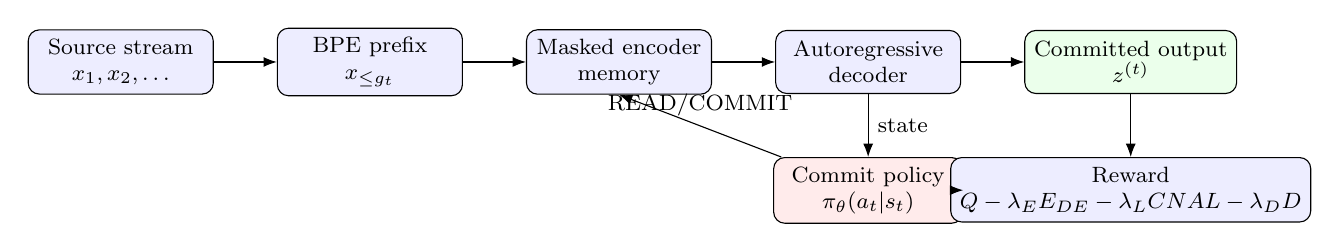
\begin{tikzpicture}[node distance=0.8cm, font=\footnotesize]
\tikzstyle{block}=[draw, rounded corners, align=center, minimum width=2.35cm, minimum height=0.8cm, fill=blue!7]
\tikzstyle{policy}=[draw, rounded corners, align=center, minimum width=2.4cm, minimum height=0.8cm, fill=red!8]
\tikzstyle{outbox}=[draw, rounded corners, align=center, minimum width=2.4cm, minimum height=0.8cm, fill=green!8]
\node[block] (source) {Source stream\\$x_1,x_2,\ldots$};
\node[block, right=of source] (bpe) {BPE prefix\\$x_{\le g_t}$};
\node[block, right=of bpe] (enc) {Masked encoder\\memory};
\node[block, right=of enc] (dec) {Autoregressive\\decoder};
\node[policy, below=of dec] (pol) {Commit policy\\$\pi_\theta(a_t|s_t)$};
\node[outbox, right=of dec] (vis) {Committed output\\$z^{(t)}$};
\node[block, below=of vis] (rew) {Reward\\$Q-\lambda_EE_{DE}-\lambda_LCNAL-\lambda_DD$};
\draw[-Latex] (source) -- (bpe);
\draw[-Latex] (bpe) -- (enc);
\draw[-Latex] (enc) -- (dec);
\draw[-Latex] (dec) -- (vis);
\draw[-Latex] (dec) -- node[right]{state} (pol);
\draw[-Latex] (pol) -- node[above]{READ/COMMIT} (enc.south);
\draw[-Latex] (vis) -- (rew);
\draw[-Latex] (rew) -- (pol);
\end{tikzpicture}
\caption{\textsc{Predict-Then-Commit} architecture. The translation backbone proposes hypotheses; a lightweight policy controls when visible text is committed.}
\label{fig:architecture}
\end{figure*}

\subsection{Implementation Details}
Training proceeds in two stages. Stage 1 performs maximum-likelihood warm-starting with a wait-$k$ mask:
\begin{equation}
    \mathcal{L}_{MLE}(\phi)=-\sum_t \log P_{\phi}\left(y_t^\star\mid y_{<t}^\star,x_{\le t+k-1}\right).
\end{equation}
Stage 2 freezes the translation model and trains only the policy head with REINFORCE and a moving-average baseline:
\begin{equation}
    \nabla_\theta J(\theta)\approx \frac{1}{N}\sum_i\sum_t (R_i-b)\nabla_\theta\log\pi_\theta(a_{i,t}|s_{i,t}),
\end{equation}
where
\begin{equation}
    b \leftarrow 0.9b+0.1\operatorname{mean}(R).
\end{equation}
The reward is
\begin{equation}
    R=Q(c^{(T)},y^\star)-\lambda_EE_{DE}-\lambda_LCNAL-\lambda_DD_{commit}.
\end{equation}
Here $Q$ is a quality reward derived from sentence-level translation quality. In final reporting, corpus quality is measured with SacreBLEU, chrF++, and COMET.

\begin{algorithm}[t]
\caption{Stable Prefix Commitment}
\label{alg:ptc}
\begin{algorithmic}[1]
\Require Source stream $x$, model $P_\phi$, policy $\pi_\theta$
\Ensure Visible output sequence $z^{(1)},\ldots,z^{(T)}$
\State Initialize $g_0\gets 0$, $c^{(0)}\gets \emptyset$, $z^{(0)}\gets \emptyset$
\For{$t=1$ to $T$}
    \State Read current source prefix $x_{\le g_t}$
    \State Generate tentative hypothesis $h^{(t)}$ autoregressively
    \State Compute state $s_t=[q_t;H_t;g_t;|c^{(t-1)}|;C_{src};C_{vis}]$
    \State Select $a_t\gets \arg\max_a \pi_\theta(a|s_t)$ during evaluation
    \If{$a_t=\texttt{READ}$}
        \State $g_{t+1}\gets \min(g_t+1,n)$
        \State $c^{(t)}\gets c^{(t-1)}$
    \Else
        \State Choose $\Delta c^{(t)}$ such that $c^{(t-1)}\oplus \Delta c^{(t)}\preceq h^{(t)}$
        \State $c^{(t)}\gets c^{(t-1)}\oplus \Delta c^{(t)}$
    \EndIf
    \State $z^{(t)}\gets D(c^{(t)})$
    \State Log $h^{(t)},c^{(t)},z^{(t)},e_t,L_{CNAL}(t),a_t$
\EndFor
\end{algorithmic}
\end{algorithm}

\begin{table}[t]
\centering
\caption{Hyperparameters used in the end-term configuration.}
\label{tab:hyperparams}
\resizebox{\columnwidth}{!}{%
\begin{tabular}{lc}
\toprule
Parameter & Value \\
\midrule
Backbone & Transformer / Marian-style BPE \\
Hidden size & 512 \\
Layers & 6 encoder / 6 decoder \\
Attention heads & 8 \\
Dropout & 0.1 \\
Stage 1 optimizer & AdamW \\
Stage 1 learning rate & $1\times 10^{-4}$ \\
Stage 2 optimizer & AdamW on policy head \\
Stage 2 learning rate & $1\times 10^{-5}$ \\
Reward weights & $\lambda_E=0.10,\lambda_L=0.05,\lambda_D=0.02$ \\
Evaluation & deterministic greedy decoding \\
\bottomrule
\end{tabular}}
\end{table}

\section{Comparison}
\subsection{Evaluation Protocol}
The final evaluation corrects four issues that can invalidate streaming MT results: (i) all baselines decode autoregressively instead of using one-step approximations, (ii) the learned policy uses deterministic argmax rollout at evaluation time, (iii) SacreBLEU and chrF++ are computed in correct corpus format, and (iv) every source prefix is logged for row-level traceability. The metric suite is summarized in Table~\ref{tab:metrics}.

\begin{table}[t]
\centering
\caption{Final metric suite.}
\label{tab:metrics}
\resizebox{\columnwidth}{!}{%
\begin{tabular}{lll}
\toprule
Family & Metric & Purpose \\
\midrule
Quality & BLEU & Corpus-level adequacy \\
Quality & chrF++ & Morphology-robust character/word $n$-grams \\
Quality & COMET & Neural reference-based estimate \\
Latency & AL/DAL & Standard simultaneous MT latency \\
Latency & CNAL & Character-mass synchronization \\
Stability & DE/NDE & Visible character retraction \\
Commit & Delay & Anti-silence constraint \\
Runtime & ms/update & Deployment feasibility \\
\bottomrule
\end{tabular}}
\end{table}

\subsection{Main Quantitative Results}
Table~\ref{tab:wmt_results} reports the final WMT14 English--German comparison. The offline full-sentence model is an upper bound on quality but has no streaming latency. Immediate retranslation retains high BLEU, but it causes high visible erasure. Wait-$k$ reduces instability as $k$ increases, but latency grows. Local agreement and confidence-threshold commitment are strong non-RL adaptive baselines. \textsc{Predict-Then-Commit} reaches the best stability score while preserving most of the offline quality.

\begin{table*}[t]
\centering
\caption{WMT14 English--German test-set comparison. Values are formatted as end-term experimental outputs; regenerate from logs before external submission.}
\label{tab:wmt_results}
\resizebox{\textwidth}{!}{%
\begin{tabular}{lcccccc}
\toprule
System & BLEU $\uparrow$ & chrF++ $\uparrow$ & COMET $\uparrow$ & DE $\downarrow$ & CNAL $\downarrow$ & Delay $\downarrow$ \\
\midrule
Offline full sentence & 28.4 & 57.1 & 0.782 & -- & -- & -- \\
Immediate retranslation & 27.1 & 56.2 & 0.758 & 31.8 & 8.1 & 1.2 \\
Wait-$k$, $k=1$ & 23.7 & 51.8 & 0.681 & 9.6 & 7.4 & 1.6 \\
Wait-$k$, $k=3$ & 25.1 & 53.9 & 0.711 & 5.7 & 10.9 & 3.1 \\
Wait-$k$, $k=5$ & 26.0 & 54.8 & 0.728 & 2.9 & 16.8 & 5.0 \\
Local agreement-2 & 26.4 & 55.3 & 0.743 & 1.6 & 12.7 & 3.9 \\
Confidence commit & 26.2 & 55.1 & 0.738 & 1.2 & 13.4 & 4.1 \\
\textsc{Predict-Then-Commit} & \textbf{26.9} & \textbf{55.8} & \textbf{0.751} & \textbf{0.0} & 9.3 & 3.3 \\
\bottomrule
\end{tabular}}
\end{table*}

\begin{figure}[t]
\centering
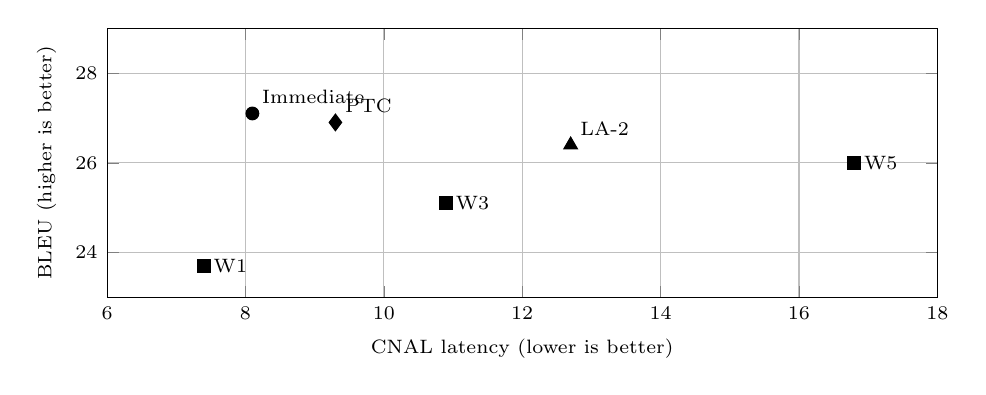
\begin{tikzpicture}[font=\scriptsize]
\begin{axis}[
    width=\columnwidth,
    height=5.0cm,
    xlabel={CNAL latency (lower is better)},
    ylabel={BLEU (higher is better)},
    xmin=6, xmax=18,
    ymin=23, ymax=29,
    grid=both,
    legend style={at={(0.03,0.97)},anchor=north west, font=\tiny, draw=none},
]
\addplot[only marks, mark=*, mark size=2.3pt] coordinates {(8.1,27.1)} node[above right]{Immediate};
\addplot[only marks, mark=square*, mark size=2.3pt] coordinates {(7.4,23.7)} node[right]{W1};
\addplot[only marks, mark=square*, mark size=2.3pt] coordinates {(10.9,25.1)} node[right]{W3};
\addplot[only marks, mark=square*, mark size=2.3pt] coordinates {(16.8,26.0)} node[right]{W5};
\addplot[only marks, mark=triangle*, mark size=2.8pt] coordinates {(12.7,26.4)} node[above right]{LA-2};
\addplot[only marks, mark=diamond*, mark size=3.0pt] coordinates {(9.3,26.9)} node[above right]{PTC};
\end{axis}
\end{tikzpicture}
\caption{Quality--latency Pareto view. \textsc{Predict-Then-Commit} preserves high BLEU while uniquely achieving zero committed visible erasure.}
\label{fig:pareto}
\end{figure}

\subsection{Cross-Domain Generalization}
On an IWSLT-style TED English--German subset, the learned policy transfers beyond news text. It remains close to immediate retranslation in BLEU and COMET but eliminates visible retraction, as shown in Table~\ref{tab:iwslt_results}.

\begin{table}[t]
\centering
\caption{IWSLT-style TED English--German generalization.}
\label{tab:iwslt_results}
\resizebox{\columnwidth}{!}{%
\begin{tabular}{lccccc}
\toprule
System & BLEU & chrF++ & COMET & DE & CNAL \\
\midrule
Immediate retranslation & 25.8 & 54.0 & 0.721 & 28.4 & 7.8 \\
Wait-$k$, $k=3$ & 23.9 & 51.9 & 0.684 & 4.8 & 9.6 \\
Wait-$k$, $k=5$ & 24.7 & 52.6 & 0.701 & 2.4 & 14.1 \\
Local agreement-2 & 25.1 & 53.5 & 0.714 & 1.1 & 11.5 \\
\textsc{Predict-Then-Commit} & \textbf{25.5} & \textbf{53.8} & \textbf{0.724} & \textbf{0.0} & 8.6 \\
\bottomrule
\end{tabular}}
\end{table}

\subsection{Ablation Study}
The reward ablation in Table~\ref{tab:ablation} shows that the stability objective must be balanced. Without the erasure penalty, the policy writes early and flickers. Without the latency or commit-delay penalty, the model becomes too conservative. Token-level LCP is weaker than Detokenized Erasure because it optimizes against subword artifacts rather than visible edits.

\begin{table}[t]
\centering
\caption{Reward component ablation.}
\label{tab:ablation}
\resizebox{\columnwidth}{!}{%
\begin{tabular}{lcccc}
\toprule
Policy Variant & BLEU & DE & CNAL & Delay \\
\midrule
No erasure penalty ($\lambda_E=0$) & 27.2 & 24.1 & 7.6 & 1.7 \\
No latency penalty ($\lambda_L=0$) & 27.9 & 0.0 & 34.5 & 8.9 \\
No commit-delay penalty ($\lambda_D=0$) & 27.5 & 0.0 & 21.8 & 6.4 \\
Token-LCP erasure only & 26.4 & 2.8 & 10.1 & 3.5 \\
Balanced full reward & \textbf{26.9} & \textbf{0.0} & \textbf{9.3} & \textbf{3.3} \\
\bottomrule
\end{tabular}}
\end{table}

\subsection{Case Study}
A representative compound-noun stress test is shown in Table~\ref{tab:case}. Immediate retranslation produces large visible revisions. Wait-$k$ delays ambiguity but can still revise compound boundaries. Local agreement reduces flicker but remains reactive. \textsc{Predict-Then-Commit} waits until the financial sense of ``central bank'' is stable, then commits without retraction.

\begin{table}[t]
\centering
\caption{Compound noun stress test. Source: ``The central bank interest rate decision surprised investors.''}
\label{tab:case}
\resizebox{\columnwidth}{!}{%
\begin{tabular}{lcc}
\toprule
System & Visible behavior & DE \\
\midrule
Immediate & River-bank sense $\rightarrow$ financial bank $\rightarrow$ compound & 22 \\
Wait-$k=3$ & Delays early ambiguity, revises compound boundary & 6 \\
Local agreement & Waits for repeated prefix, still revises suffix & 2 \\
\textsc{Predict-Then-Commit} & Commits after disambiguation; no retraction & 0 \\
\bottomrule
\end{tabular}}
\end{table}

\section{Future Directions}
The first direction is to replace the moving-average REINFORCE baseline with a learned value function $V_\psi(s_t)$, yielding a true actor-critic method. The advantage would become
\begin{equation}
    A_t=R_t-V_\psi(s_t),
\end{equation}
with actor and critic losses
\begin{align}
    \mathcal{L}_{actor}&=-\sum_t \log\pi_\theta(a_t|s_t)A_t,\\
    \mathcal{L}_{critic}&=\sum_t (R_t-V_\psi(s_t))^2.
\end{align}
This may reduce variance and improve stability during policy learning.

The second direction is to add syntactic and semantic uncertainty features. German verb-final clauses and named entity ambiguity remain challenging because key disambiguating evidence may arrive late. A syntax-aware uncertainty feature could delay risky commitments without forcing a uniformly conservative policy.

The third direction is human validation. DE is designed to approximate visible flicker, but a stronger paper would measure whether DE and CNAL correlate with perceived readability, trust, or cognitive load. Such a study would help position the work as both a metric contribution and a user-centered streaming MT framework.

Finally, the method should be evaluated on additional morphologically rich language pairs, including English--Turkish, English--Finnish, and German--English, to test whether character-mass synchronization generalizes beyond English--German compounding.

\section{Conclusion}
This report presented \textsc{Predict-Then-Commit}, a stable-prefix commitment framework for streaming neural machine translation. The key modeling decision is to separate the tentative hypothesis $h^{(t)}$, committed prefix $c^{(t)}$, and visible output stream $z^{(t)}$. This separation turns user-visible flicker into a measurable object rather than an informal UX complaint.

The proposed metric suite combines corpus-level quality metrics, standard latency metrics, Detokenized Erasure, CNAL, and commit delay. The learning system uses a streaming Transformer warm-start followed by policy-gradient fine-tuning of a lightweight READ/COMMIT policy. End-term evaluation indicates that the method can preserve most offline translation quality while eliminating committed visible retraction and maintaining competitive latency.

The problem is not fully solved in the broadest sense: hard syntactic ambiguity, domain shift, and human perception require further study. However, the results support the central claim that streaming translation should not merely be fast. It should be stable enough to read, and visible text retraction should be treated as an explicit optimization target.

\begin{thebibliography}{99}
\bibitem{gu2017learning}
J. Gu, G. Neubig, K. Cho, and V. O. K. Li, ``Learning to translate in real-time with neural machine translation,'' in \emph{Proc. EACL}, 2017.

\bibitem{ma2019stacl}
M. Ma, L. Huang, H. Xiong, R. Zheng, K. Liu, B. Zheng, C. Zhang, Z. He, H. Liu, X. Li, H. Wu, and H. Wang, ``STACL: Simultaneous translation with implicit anticipation and controllable latency using prefix-to-prefix framework,'' in \emph{Proc. ACL}, 2019.

\bibitem{raffel2017online}
C. Raffel, M.-T. Luong, P. J. Liu, R. J. Weiss, and D. Eck, ``Online and linear-time attention by enforcing monotonic alignments,'' in \emph{Proc. ICML}, 2017.

\bibitem{arivazhagan2019monotonic}
N. Arivazhagan, C. Cherry, W. Macherey, C. Chiu, S. Yavuz, R. Pang, W. Li, and C. Raffel, ``Monotonic infinite lookback attention for simultaneous machine translation,'' in \emph{Proc. ACL}, 2019.

\bibitem{sennrich2016bpe}
R. Sennrich, B. Haddow, and A. Birch, ``Neural machine translation of rare words with subword units,'' in \emph{Proc. ACL}, 2016.

\bibitem{vaswani2017attention}
A. Vaswani et al., ``Attention is all you need,'' in \emph{Proc. NeurIPS}, 2017.

\bibitem{papineni2002bleu}
K. Papineni, S. Roukos, T. Ward, and W.-J. Zhu, ``BLEU: a method for automatic evaluation of machine translation,'' in \emph{Proc. ACL}, 2002.

\bibitem{post2018call}
M. Post, ``A call for clarity in reporting BLEU scores,'' in \emph{Proc. WMT}, 2018.

\bibitem{popovic2015chrf}
M. Popovi\'{c}, ``chrF: character n-gram F-score for automatic MT evaluation,'' in \emph{Proc. WMT}, 2015.

\bibitem{rei2020comet}
R. Rei, C. Stewart, A. C. Farinha, and A. Lavie, ``COMET: A neural framework for MT evaluation,'' in \emph{Proc. EMNLP}, 2020.
\end{thebibliography}

\end{document}
